\chapter{Конструкторская часть}

В данном разделе будут описаны сущности и построена диаграмма базы данных. 
Также будет формализована ролевая модель на уровне базы данных и описаны проектируемые функции.

\section{Сущности базы данных}

На рисунке \ref{img:newDB} представлена диаграмма разрабатываемой базы данных.

\begin{figure}[h]
    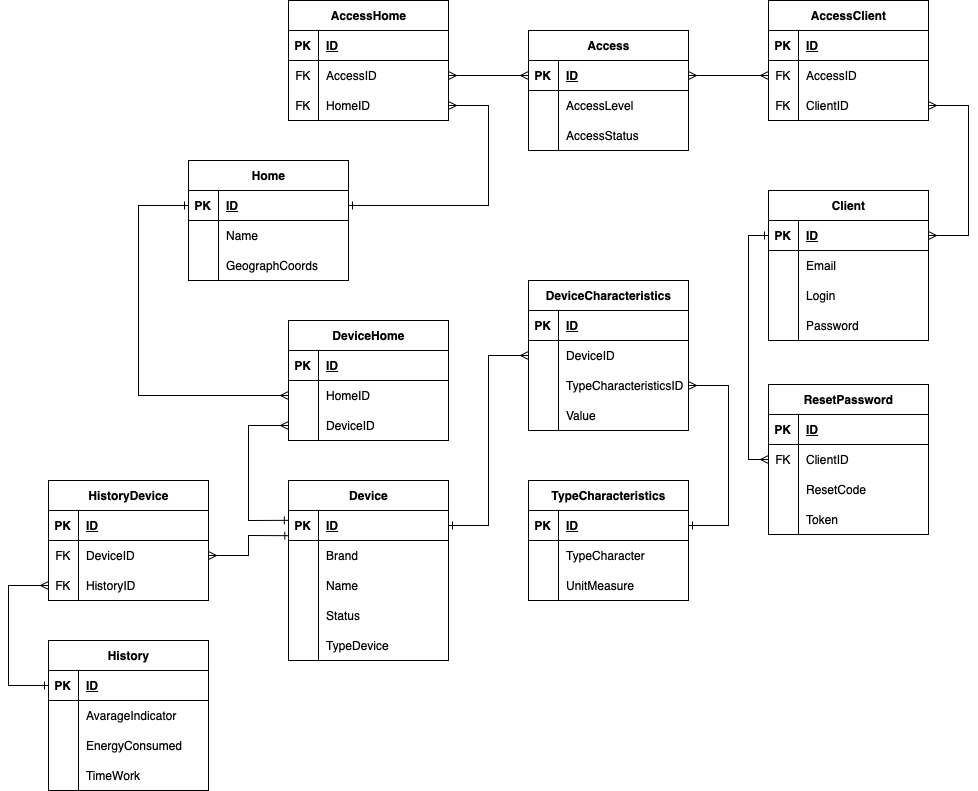
\includegraphics[width=0.9\linewidth]{img/newDB.png}
    \caption{\label{img:newDB} Диаграмма разрабатываемой базы данных}
\end{figure}
\noindent
\clearpage

На диаграмме представлены следующие таблицы:

\begin{enumerate}
    \item[1)] Client -- таблица, содержащая информацию о клиентах, 
    состоит из следующих компонентов:
    \begin{itemize}
        \item ID -- уникальный идентификатор(serial4), первичный ключ таблицы;
        \item Email -- почта пользователя (символьный тип c переменным значением, непустая строка);
        \item Login -- логин пользователя (символьный тип c переменным значением, непустая строка);
        \item Password -- пароль пользователя (символьный тип c переменным значением, непустая строка), который 
        в базе данных хранится как хешированная строка.
    \end{itemize}
    \item[2)] Access -- таблица привилегий доступа, содержащая:
    \begin{itemize}
        \item ID -- уникальный идентификатор(serial4), первичный ключ таблицы;
        \item AccessLevel -- уровень доступа пользователя к дому;
        \item AccessStatus -- текущий доступ к системе умного дома.
    \end{itemize}
    \item[3)] AccessClient -- таблица, которая реализует отношение 
    «один-ко-многим» между таблицами «Client» и «Access», 
    имеет два уникальных идентификатора (клиент и доступ).
    \item[4)] Home -- таблица, предоставляющая информацию о домах, содержит следующие поля:
    \begin{itemize}
        \item ID -- уникальный идентификатор(serial4), первичный ключ таблицы;
        \item Name -- имя дома;
        \item GeographCoords -- географические координаты, показывающие расположение дома.
    \end{itemize}
    \item[5)] AccessHome -- таблица, которая реализует отношение 
    «один-ко-многим» между таблицами «Home» и «Access»,
    имеет два уникальных идентификатора (дом и доступ).
    \item[6)] Device -- таблица, предоставляющая информацию об устройствах, содержит следующие поля:
    \begin{itemize}
        \item ID -- уникальный идентификатор(serial4), первичный ключ таблицы;
        \item Name -- имя устройства;
        \item Brand -- бренд устройства;
        \item Status -- текущее состояние устройства;
        \item TypeDevice -- тип устройства.
    \end{itemize}
    \item[7)] DeviceHome -- таблица, которая реализует отношение 
    «многие-ко-многим» между таблицами «Device» и «Home»,
    имеет два уникальных идентификатора (устройство и дом).
    \item[8)] History -- таблица, содержащая историю работы устройств, имеет следующие поля:
    \begin{itemize}
        \item ID -- уникальный идентификатор(serial4), первичный ключ таблицы;
        \item AvarageIndicator -- средний показатель характеристики устройства;
        \item EnergyConsumed -- потребленная энергия устройством за время работы;
        \item TimeWork -- время работы устройства.
    \end{itemize}
    \item[9)] HistoryDevice -- таблица, которая реализует отношение 
    «многие-ко-многим» между таблицами «Device» и «History»,
    имеет два уникальных идентификатора (устройство и история).
    \item[10)] ResetPassword -- таблица, которая необходима для восстановления пароля пользов ателя, она содержит:
    \begin{itemize}
        \item ID -- уникальный идентификатор(serial4), первичный ключ таблицы;
        \item ClientID -- уникальный идентификатор пользователя, который восстанавливает пароль;
        \item ResetCode -- код, необходимый для подтверждения проверки пользователя;
        \item Token - токен доступа.
    \end{itemize}
        
    
\end{enumerate}

\section{Функции базы данных}

Когда устройство начинает работать, необходимо обновлять 
статус для того, чтобы пользователь
мог увидеть текущее состояние устройства. 
Для этого была описана функция, которая после окончания работы
обновляет статус устройства с «Active» на «Inactive» и 
при запуске устройства с «Inactive» на «Active». 
Схема алгоритма данной функции указана на следующем рисунке
\ref{pic:func1}:

\begin{figure}[h]
    \centering 
    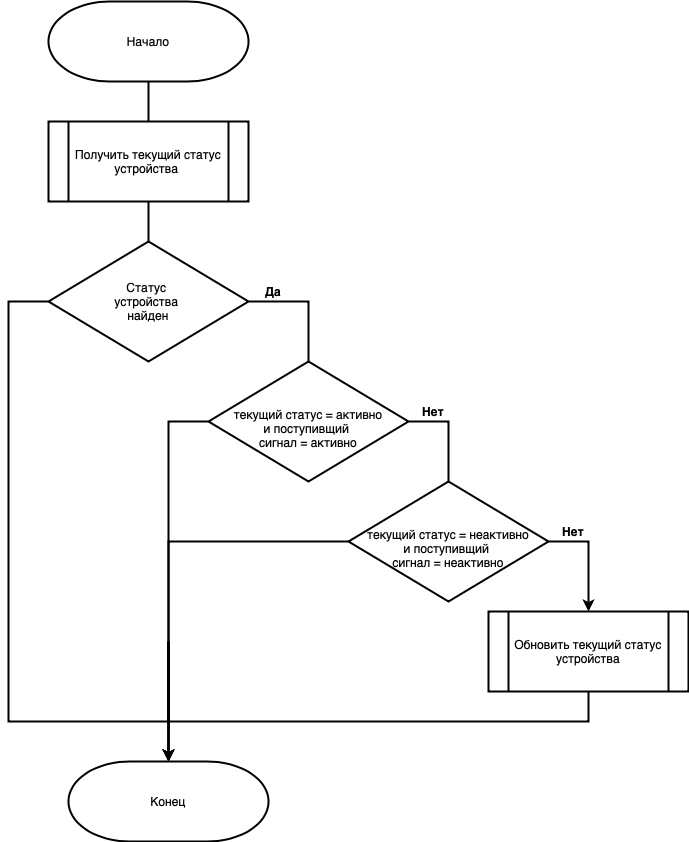
\includegraphics[width=0.6\linewidth]{img/updatestatusfunc.png}
    \caption{ER-диаграмма в нотации Чена}
    \label{pic:func1}
\end{figure}
\noindent
\clearpage

\section{Роли базы данных}

Для управления доступом к таблицам применяются роли. 
В аналитической части были установлены следующие роли: 
гость (неавторизованный пользователь), авторизованный 
пользователь, владелец дома и участник дома. 
Для каждой из этих ролей необходимо разработать 
соответствующие права доступа:
\begin{enumerate}
    \item[1)] гость(неавторизованный пользователь) должен
    иметь доступ на изменение и просмотр данных в таблице «Client»;
    \item[2)] авторизованный пользователь имеет все права
    гостя, так же ему предоставлены изменение и добавление данных
    в таблицу «Home»;
    \item[3)] участник дома должен иметь все права авторизованного 
    пользователя, так же ему доступен просмотр таблиц
    «History», «Device», «TypeCharacteristics», «Access», в зависимости
    от предоставленных прав владельцем дома участнику может быть
    доступно добавление, изменение данных в указанных таблицах;
    \item[3)] владелец должен иметь возможность 
    просматривать и изменять записи во всех существующих таблицах.
\end{enumerate}

\section*{Вывод}

В данном разделе были описаны сущности и построена диаграмма
базы данных, описана ипользуемая функция и приведена схема ее алгоримта.
Так же были формализованы роли на уровене базы
данных, чтобы обеспечить управление доступом к таблицам.
